\documentclass{beamer}
%\documentclass[handout]{beamer}
\usepackage[hungarian]{babel}
\uselanguage{hungarian}
\languagepath{hungarian}
\deftranslation[to=hungarian]{Theorem}{T\'etel}
\deftranslation[to=hungarian]{Example}{P\'elda}
\deftranslation[to=hungarian]{Definition}{Defin\'ici\'o}
%\usepackage[magyar]{babel}
\usepackage[utf8]{inputenc}
\usepackage[T1]{fontenc}
\usepackage{beamerthemesplit}
\usepackage{pgf,pgffor,pgfplots}
\pgfplotsset{compat=1.15}
\usepackage{subfig}
\usepackage{xcolor}
\usepackage{listings}

\usepackage{xcolor}

\makeatletter
\let\old@lstKV@SwitchCases\lstKV@SwitchCases
\def\lstKV@SwitchCases#1#2#3{}
\makeatother
\usepackage{lstlinebgrd}
\makeatletter
\let\lstKV@SwitchCases\old@lstKV@SwitchCases

\lst@Key{numbers}{none}{%
	\def\lst@PlaceNumber{\lst@linebgrd}%
	\lstKV@SwitchCases{#1}%
	{none:\\%
		left:\def\lst@PlaceNumber{\llap{\normalfont
				\lst@numberstyle{\thelstnumber}\kern\lst@numbersep}\lst@linebgrd}\\%
		right:\def\lst@PlaceNumber{\rlap{\normalfont
				\kern\linewidth \kern\lst@numbersep
				\lst@numberstyle{\thelstnumber}}\lst@linebgrd}%
	}{\PackageError{Listings}{Numbers #1 unknown}\@ehc}}
\makeatother


\AtBeginEnvironment{figure}{\setcounter{subfigure}{0}}
\makeatletter
%%%%%%%%%%%%%%%%%%%%%%%%%%%%%%%%%%%%%%%%%%%%%%%%%%%%%%%%%%%%%%%%%%%%%%%%%%%%%%
%
% \btIfInRange{number}{range list}{TRUE}{FALSE}
%
% Test in int number <number> is element of a (comma separated) list of ranges
% (such as: {1,3-5,7,10-12,14}) and processes <TRUE> or <FALSE> respectively

\newcount\bt@rangea
\newcount\bt@rangeb

\newcommand\btIfInRange[2]{%
    \global\let\bt@inrange\@secondoftwo%
    \edef\bt@rangelist{#2}%
    \foreach \range in \bt@rangelist {%
        \afterassignment\bt@getrangeb%
        \bt@rangea=0\range\relax%
        \pgfmathtruncatemacro\result{ ( #1 >= \bt@rangea) && (#1 <= \bt@rangeb) }%
        \ifnum\result=1\relax%
            \breakforeach%
            \global\let\bt@inrange\@firstoftwo%
        \fi%
    }%
    \bt@inrange%
}
\newcommand\bt@getrangeb{%
    \@ifnextchar\relax%
        {\bt@rangeb=\bt@rangea}%
        {\@getrangeb}%
}
\def\@getrangeb-#1\relax{%
    \ifx\relax#1\relax%
        \bt@rangeb=100000%   \maxdimen is too large for pgfmath
    \else%
        \bt@rangeb=#1\relax%
    \fi%
}

%%%%%%%%%%%%%%%%%%%%%%%%%%%%%%%%%%%%%%%%%%%%%%%%%%%%%%%%%%%%%%%%%%%%%%%%%%%%%%
%
% \btLstHL<overlay spec>{range list}
%
% TODO BUG: \btLstHL commands can not yet be accumulated if more than one overlay spec match.
% 
\newcommand<>{\btLstHL}[1]{%
  \only#2{\btIfInRange{\value{lstnumber}}{#1}{\color{orange!30}\def\lst@linebgrdcmd{\color@block}}{\def\lst@linebgrdcmd####1####2####3{}}}%
}%
\makeatother



\usepackage{hyperref}
\hypersetup{
    colorlinks = true,
    linkcolor = blue,
    urlcolor  = blue,
    citecolor = blue,
    linkbordercolor = {white},
}
\usepackage{alltt}
\usepackage{tikz}
\usetikzlibrary{trees}
\usetikzlibrary{shapes,shapes.geometric,shapes.multipart}
\usetikzlibrary{calc,chains,arrows,positioning}
\tikzset{
  box/.style={draw, fill=pink!10, minimum width=5em, text centered, minimum height=2.5em},
  treenode/.style = {circle, draw, align=center, inner sep=3pt, text centered, font=\sffamily, text width=1em},
  int/.style = {rectangle split,rectangle split parts=2,draw,text centered, text width = 1.6cm, text height = 0.3cm},
  subtree/.style={isosceles triangle, draw=black, align=center, minimum height=0.5cm, minimum width=1cm, shape border rotate=90, anchor=north},
  data/.style={
      minimum width=2em,
      minimum height=2em,
      draw, rectangle split,
      rectangle split parts=2, text centered,
  }
}

\usetheme{Warsaw}
\institute{Szegedi Tudományegyetem}
\pgfdeclareimage[height=0.55cm]{institution-logo}{../szte_logo}
\logo{\pgfuseimage{institution-logo}}

\title{Algoritmusok és adatszerkezetek II.}
\subtitle{Kiegyensúlyozott keresőfák}
\date{}

\begin{document}

\maketitle

\begin{frame}{Mit értünk kiegyensúlyozott keresőfa alatt?}
	\begin{beamerboxesrounded}{Emlékeztető}
Az eddig tárgyalt műveletek $h$ magas fákra $O(h)$ idejűek voltak \\
A továbbiakban szeretnénk, ha $h=\Theta(\log n)$ is teljesülne
	\end{beamerboxesrounded}
    \begin{columns}
    	\begin{column}{.5\linewidth}
\begin{figure}[!h]
\centering
    \begin{tikzpicture}[scale=.5, level/.style={sibling distance = 3cm}]
    \node[treenode]{1}
		child[missing]
    	child{ node[treenode] {2}
			child[missing]
    		child{ node[treenode] {3}
				child[missing]
    			child{ node[treenode] {4}
					child[missing]
	    			child{ node[treenode] {5}
						child[missing]
		    			child{ node[treenode] {6}
							child[missing]
			    			child{ node[treenode] {7}}
		    			}
	    			}
    			}
    		}
    	};
\end{tikzpicture}
\end{figure}
    	\end{column}
    	\begin{column}{.5\linewidth}
\begin{figure}
\centering
    \begin{tikzpicture}[scale=.5, level 1/.style={sibling distance=6cm}, level 2/.style={sibling distance=3cm}]
    \node[treenode]{4}
    	child{ node[treenode] {2}
			child{node[treenode] {1}}
			child{node[treenode,level distance=3cm] {3}}
    	}
    	child{ node[treenode] {6}
			child{node[treenode] {5}}
			child{node[treenode] {7}}
    	};
\end{tikzpicture}
\end{figure}
    	\end{column}
    \end{columns}
\end{frame}

\begin{frame}{Véletlen építésű bináris keresőfák (CLRS 12.4)}
	\begin{itemize}
		\item $n$ elemű bináris fa \textbf{legrosszabb esetben} $\Theta(n)$ magas is lehet
		\item $n$ növekedésével a legrosszabb eset bekövetkezése azonban egyre valószínűtlenebb
		\item Ha egy bináris keresőfa előállítása során csak beszúrás műveleteket alkalmazunk, úgy igazolható a következő
	\end{itemize}
	\begin{theorem}
Egy n különböző kulcsot tartalmazó véletlen építésű bináris keresőfa várható magassága $O(\log n)$.
	\end{theorem}
\end{frame}

\section{AVL fa}
\begin{frame}{AVL fák (Adelson-Velsky, Landis, 1962)}
    \begin{itemize}
    	\item \textbf{Tetszőleges} műveletsorozat végrehajtása után \textbf{legrosszabb esetben is} $\Theta(\log n)$ magasságú kiegyensúlyozott keresőfa
    	\item Garancia: semelyik csúcs egyensúlyi faktorának abszolút értéke nem lehet nagyobb 1-nél
    	\begin{definition}
    	Egy $p$ csúcs \textbf{egyensúlyi faktor}a fiai magasságának különbsége.
    	\end{definition}
		\begin{definition}
    	 Üres fa magassága: $h(nil)=0$\\
    	 $p$ gyökerű fa magassága: $h(p)=max(h(p.bal), h(p.jobb))+1$
    	\end{definition}
    \end{itemize}
\end{frame}

\begin{frame}[fragile]{AVL fa implementációja}
	\begin{columns}
		\begin{column}{.7\textwidth}
\begin{lstlisting}[
  linebackgroundcolor={
    \btLstHL<1->{3}
  }]
class Node {
    Object kulcs;
    int magassag;
    Node *apa;
    Node *bal;
    Node *jobb;
}
\end{lstlisting}
			\begin{block}<2>{Megjegyzés}
				Találkozni olyan implementációval is, ahol a magasság helyett 
				az egyensúlyi faktort tárolják
			\end{block}

		\end{column}
		
		\begin{column}{.4\textwidth}
		\begin{figure}
		\centering
\begin{tikzpicture}[node distance=0cm,outer sep = 0pt]
    \node (A) [box,minimum width=6em] {kulcs};
    \node (H) [box,anchor=north,minimum width=6em,fill=orange!30] at (A.south) 
    {magassag};
    \node (D) [box,anchor=south,minimum width=6em] at (A.north) {apa};
    \node (B) [box,anchor=north west,minimum width=3em] at (H.south west) {bal};
    \node (C) [box,anchor=north east,minimum width=3em] at (H.south east) 
    {jobb};
    \coordinate (E) at (0,2);
    \coordinate (E) at (0,2);
    \node[below left = 1cm of B] (F) {};
    \node[below right = 1cm of C] (G) {};
%    \path (D) edge [->] node[pos=0.5,anchor=-135,inner sep=1pt] {N} (E);
    \path (D) edge [->] (E);
    \path (B) edge [->] (F);
    \path (C) edge [->] (G);
\end{tikzpicture}
		\end{figure}
		\end{column}
	\end{columns}
\end{frame}

\begin{frame}{Legalább hány kulcsból áll egy $h$ magas AVL fa?}
	\begin{table}
		\centering
		\begin{tabular}{c|c}
			magasság & $m$ \\ \hline
			1 & 1     \\
			2 & 2     \\
		    3 & 1+2+1=4 \\
			4 & 2+4+1=7 \\
			5 & 4+7+1=12 \\
			6 & 7+12+1=20 \\
			7 & 12+20+1=33 \\
			8 & 20+33+1=54 \\
		    \vdots & \vdots \\
		    \pause h & $m_{h-2}+m_{h-1}+1$
		\end{tabular}
	\end{table}
%	\begin{block}{Fibonacci sor}
%	$F_1=F_2=1$, továbbá $F_i=F_{i-2}+F_{i-1}$, $i>2$ esetén \\
%	1,1,2,3,5,8,13,21,34,55
%	\end{block}
\end{frame}

\begin{frame}{Miért igaz, hogy az AVL fák $O(\log n)$ magasak?}
	\begin{itemize}
		\item Jelölje $m_h$ a $h$ magas AVL fában lévő minimálisan található kulcsok számát ($m_1=1, m_2=2$)
		\item Általánosságban ($h>2$ esetén): $m_h=m_{h-2}+m_{h-1}+1$
		\item $m_{h-2} < m_{h-1}$ természetesen teljesül, ahonnan \only<1>{$$m_h > 2 m_{h-2}\vphantom{>2*2 m_{h-4}>\ldots>2^i m_{h-2i}}$$}\only<2->{$$m_h > 2 m_{h-2}>2*2 m_{h-4}>\ldots>2^i m_{h-2i}$$}
		\item<3-> $m_{h} > 2^i m_{h-2i}$ összefüggést $m_1$-ig kijátszva $m_{h} > 2^{h/2}$
		\item<4-> Tegyük fel, hogy egy $h$ magas AVL fa $n \geq m_h$ csúcsból áll, azaz $n > 2^{h/2}$, vagyis $h < 2 \log_2(n)$
	\end{itemize}
	\pause[5]
		\begin{block}{Megjegyzés}
		Az élesebb $h < 1.44 \log_2(n)$ korlát is bizonyítható.
		\end{block}
\end{frame}

\begin{frame}{AVL fák kiegyensúlyozottságának fenntartása forgatásokkal}
    \begin{figure}
    \subfloat[\only<1>{beszúrás előtt}\only<2->{beszúrás után}]{
      \begin{tikzpicture}[scale=.9,level/.style={sibling distance = 2.4cm},level distance=1.4cm]
          \node[data,minimum width=1cm]{x \nodepart{two}\only<1>{h}\only<2->{\textcolor{red}{h+1}}}
              child{ node[subtree]{$\alpha$\\ h-2}
              }
              child{ node[data]{y \nodepart{two}\only<1>{h-1}\only<2->{\textcolor{red}{h}}}
                  child{ node[subtree]{$\beta$\\ h-2}}
                  child{ node[subtree]{$\gamma$\\ \only<1>{h-2}\only<2->{\textcolor{red}{h-1}}}}
              };
        \end{tikzpicture}
    } \hfill
    \only<2->{
    \subfloat[$x$ körüli balra forgatva]{
    	\begin{tikzpicture}[scale=.9,level/.style={sibling distance =2.4cm},level distance=1.4cm]
    		\node[data]{y \nodepart{two} \only<-2>{\phantom{h}}\only<-2>{\phantom{h}}\only<3>{h}}
    		child{ node[data]{x \nodepart{two} \only<-2>{\phantom{h-1}}\only<3>{h-1}}
    		                  child{ node[subtree]{$\alpha$\\ \only<-2>{\phantom{h-2}}\only<3>{h-2}}}
    		                  child{ node[subtree]{$\beta$\\ \only<-2>{\phantom{h-2}}\only<3>{h-2}}}
    		 }
            child{ node[subtree]{$\gamma$\\\only<-2>{\phantom{h-1}}\only<3>{h-1}}}
            ;
            \end{tikzpicture}
        }
    }
    \end{figure}
\end{frame}

\begin{frame}{Amikor egy forgatás nem elég}
    \begin{figure}
    \subfloat[\only<1>{beszúrás előtt}\only<2->{beszúrás után}]{
      \begin{tikzpicture}[scale=.9,level/.style={sibling distance = 2.4cm},level distance=1.4cm]
          \node[data, minimum width=1cm]{x \nodepart{two}\only<1>{h}\only<2->{\textcolor{red}{h+1}}}
              child{ node[subtree]{$\alpha$\\ h-2}
              }
              child{ node[data]{y \nodepart{two}\only<1>{h-1}\only<2->{\textcolor{red}{h}}}
                  child{ node[subtree]{$\beta$\\ \only<1>{h-2}\only<2->{\textcolor{red}{h-1}}}}
                  child{ node[subtree]{$\gamma$\\ h-2 }}
              };
        \end{tikzpicture}
    } \hfill
    \only<2->{
    \subfloat[$x$ körüli balra forgatva]{
    	\begin{tikzpicture}[scale=.9,level/.style={sibling distance =2.4cm},level distance=1.4cm]
    		\node[data]{y \nodepart{two} \only<-2>{\phantom{h+1}}\only<3>{h+1}}
    		child{ node[data]{x \nodepart{two} \only<-2>{\phantom{\textbf{h}}}\only<3>{\textcolor{red}{\textbf{h}}}}
    		                  child{ node[subtree]{$\alpha$\\ \only<-2>{\phantom{h-2}}\only<3>{h-2}}}
    		                  child{ node[subtree]{$\beta$\\ \only<-2>{\phantom{h-1}}\only<3>{h-1}}}
    		 }
            child{ node[subtree]{$\gamma$\\\only<-2>{\phantom{\textbf{h-2}}}\only<3>{\textcolor{red}{\textbf{h-2}}}}}
            ;
            \end{tikzpicture}
        }
    }
    \end{figure}
\end{frame}

\begin{frame}{Amikor egy forgatás nem elég -- segédforgatás}
\begin{columns}
\begin{column}{.6\linewidth}
    \begin{figure}
      \begin{tikzpicture}[level/.style={sibling distance =3cm}, level 1/.style={sibling distance=2.5cm}, level 2/.style={sibling distance=2.5cm}]
          \node[data]{x \nodepart{two}h+1}
              child{ node[subtree, color=red]{$\alpha$\\ h-2}
              }
              child{ node[data,color=red]{y \nodepart{two}h}
                  child{ node[data]{z \nodepart{two} h-1}
                     child{node[subtree]{$\beta_1$ \\ \tiny{< h-1}}}
                     child{node[subtree]{$\beta_2$ \\ \tiny{< h-1} }}}
                  child{ node[subtree]{$\gamma$\\ h-2 }}
              };
        \end{tikzpicture}
    \end{figure}
\end{column}
\begin{column}{.5\linewidth}
    \begin{alertblock}{Megoldás}
    $y$ körül jobbra forgatunk, majd $x$ körül balra
    \end{alertblock}
\end{column}
\end{columns}
\end{frame}

\begin{frame}{Amikor egy forgatás nem elég -- segédforgatás}
\begin{columns}
\begin{column}{.6\linewidth}
    \begin{figure}
		\begin{tikzpicture}[level/.style={sibling distance =3cm}, level 1/.style={sibling distance=2.5cm}, level 2/.style={sibling distance=1.5cm}]
          \node[data]{x \nodepart{two}h+1}
              child{ node[subtree, color=red]{$\alpha$\\ h-2}
              }
              child{ node[data, color=red]{z \nodepart{two} h}
              	child{node[subtree]{$\beta_1$ \nodepart{two}}}
                child{node[data]{y \nodepart{two} h-1}
                	child{node[subtree]{$\beta_2$}}
                    child{node[subtree]{$\gamma$ \\ h-2}}
                  }
              };
        \end{tikzpicture}
    \end{figure}
\end{column}
\begin{column}{.5\linewidth}
    \begin{block}{Észrevétel}
    $\beta_2$ nem lehetett magasabb $\gamma$-nál
    \end{block}
\end{column}
\end{columns}
\end{frame}

\begin{frame}{Amikor egy forgatás nem elég -- segédforgatás}
\begin{columns}
\begin{column}{.6\linewidth}
    \begin{figure}
		\begin{tikzpicture}[level/.style={sibling distance =3cm}, level 1/.style={sibling distance=3cm}, level 2/.style={sibling distance=1.5cm}]
          \node[data]{z \nodepart{two}h}
                child{node[data]{x \nodepart{two} h-1}
                	child{node[subtree]{$\alpha$ \\ h-2}}
                    child{node[subtree]{$\beta_1$}}
                  }
                child{ node[data]{y \nodepart{two} h-1}
                	child{node[subtree]{$\beta_2$}}
                    child{node[subtree]{$\gamma$ \\ h-2}}
              };
        \end{tikzpicture}
    \end{figure}
\end{column}
\begin{column}{.5\linewidth}
\begin{block}{Miért kellett kettőt forgassunk?}
Mert (kiinduláskor) $x$ \textbf{jobboldali} részfája volt magasabb \\
És mert ennek a részfának már a \textbf{baloldali} részfája volt magasabb (zikk-zakk)
\end{block}
\end{column}
\end{columns}
\end{frame}

\begin{frame}{Megjegyzések a helyreállításokhoz}
\begin{itemize}
    \item A tárgyalt esetek tükörképei is előfordulhatnak
    \item A törlés hatására elromló AVL-fát azonos módon állítjuk helyre
\end{itemize}
\end{frame}

\begin{frame}{Általános keresőfák}
\begin{itemize}
\item Az általános keresőfát az különbözteti meg a bináris keresőfától, hogy egy csúcs több kulcsot is tartalmazhat
\item Keresőfa tulajdonság kiterjesztése
\begin{itemize}
\item A csúcsban található kulcsok $<$ szerint rendezettek
\item A tárolt kulcsok értékei meghatározzák a kulcsértékeknek azon tartományait, amelyekbe a részfák kulcsai eshetnek
\end{itemize}
\end{itemize}
\begin{example}<2>
	\begin{figure}
		\centering
		\begin{tikzpicture}
			\tikzstyle{bnode}=[rectangle split, rectangle split parts=3, rectangle split horizontal,rectangle split ignore empty parts,draw, fill=white]
			\tikzstyle{every node}=[bnode]
			\tikzstyle{level 1}=[sibling distance=3cm,level distance=2cm]
			\node {22 \nodepart{two} 65}
				child {node{3}  edge from parent node[sloped,anchor=south,auto=false,draw=none] {\tiny x<22}}
				child {node{26 \nodepart{two} 35 \nodepart{three} 58} edge from parent node[anchor=south,auto=false,draw=none] {\tiny 22<x<65}}
				child {node{76 \nodepart{two} 80 \nodepart{three} 98}  edge from parent node[sloped,anchor=south,auto=false,draw=none] {\tiny 65<x}
			};
		\end{tikzpicture}
	\end{figure}
\end{example}
\end{frame}

\section{B-fa}

\begin{frame}{B-fa definíciója}
	\begin{definition}
		A $t$-rendű B-fa olyan általános keresőfa, amelyre teljesül, hogy:\\
		\begin{itemize}
			\item Minden gyökértől különböző $p$ csúcsára $t \leq Rang(p) \leq 2t$ (rang alatt a fapontban tárolt kulcsok számát értjük)
			\item $r$ gyökerének rangjára pedig $1 \leq Rang(r) \leq 2t$ \\
			\item Minden nemlevél $p$ csúcsra és $1 \leq i \leq Rang(p)+1$ esetén $p.gyerekek[i] \neq Nil$
			\item Minden levél azonos mélységű (ez az érték a fa $h$ magassága).
		\end{itemize}
	\end{definition}
\end{frame}

\begin{frame}[fragile]{B-fa implementációja}
\begin{lstlisting}[
  linebackgroundcolor={
    \btLstHL<1->{2-3,5-6}
  }]
class Node {
    Object[] kulcsok;
    int meret;
    Node *apa;
    Node *gyerekek[meret+1];
    boolean level;
}
\end{lstlisting}
			\begin{alertblock}<2>{Fontos!}
				Az eddigiektől eltérően egy csúcsban több kulcs is található. \\
				A csúcson belüli kulcsokra érvényesül a $<$ rendezés. \\
				A csúcsokról eltároljuk, hogy levelek-e (\texttt{level} változó)
			\end{alertblock}
\end{frame}

\begin{frame}[fragile]{B-fában keresés}
\begin{alltt}
{\scshape B-FábanKeres}(x, k) \{
   i=0
   while i < meret és k > x.kulcsok[i] \{
      i = i+1
   \}

   if (i < meret és k = x.kulcsok[i]) \{
      return (x,i)   // az x csúcs i-edik kulcsát kerestük
   if (x.level) \{
      return nil    // a B-fa nem tartalmazza k-t
   \} else \{
      // a megfelelő ágban keresünk tovább
      return {\scshape B-FábanKeres}(x.gyerekek[i], k)
   \}
 \}
\end{alltt}
\end{frame}

\begin{frame}{B-fák kiegyensúlyozottsága}
	\begin{itemize}
		\item B fákat olyan esetekben szokás használni, amikor az adatunk nem fér be a főmemóriába, azt a háttértáron tároljuk
		\item A B-fák kiegyensúlyozottsága abból fakad, hogy minden levél azonos mélységen található, illetve, hogy minden (nemgyökér) csúcs legalább $t+1$ elágazással rendelkezik
		\begin{itemize}
			\item $t$-rendű B-fa $i$-edik ($i>1$) szintjén legalább $2 (t+1)^{i-2}$ csúcs és $2t (t+1)^{i-2}$ érték található \
			\item $t$ értéke a valóságban nagy, mi ezen a kurzuson $2$-nek vesszük (hacsak mást nem mondunk)
		\end{itemize}		
		\item Az AVL-fánál ''kiegyensúlyozottabb'', magassága $O(\log_{{\color{red} \textbf{t}}} n)$
		\begin{itemize}
			\item Aszimptotikusan nincs jelentősége a logaritmus alapjának, viszont ha másodlagos memóriából olvasunk, számíthat
		\end{itemize}
	\end{itemize}
\end{frame}

\begin{frame}{B-fák tulajdonságainak fenntartása -- méret túlcsordulása}
	\begin{itemize}
	    \item B-fákba is levélként szúrunk be
		\item $2t$ méretű csúcsba beszúrva, $2t+1$ méretű csúcsot kapunk \pause a ''középső'' elem mentén kettévágva éppen 2 $t$ méretű csúcsunk lesz (a középső elemet küldjük föl az ősbe)
		\item Szükség szerint ismételjük az előző lépést
	\end{itemize}
	\begin{example}<2->
	    \only<2>{
		\begin{figure}
			\centering
			\begin{tikzpicture}
				\tikzstyle{bnode}=[rectangle split, rectangle split parts=4, rectangle split horizontal,rectangle split ignore empty parts,draw, fill=white]
				\tikzstyle{every node}=[bnode]
				\tikzstyle{level 1}=[sibling distance=3cm,level distance=1cm]
				\node {22 \nodepart{two} 65}
					child {node{3  \nodepart{two} 19 }}
					child {node{26 \nodepart{two} 35 \nodepart{three} 58}}
					child {node{76 \nodepart{two} 78 \nodepart{three} 80 \nodepart{four} 90}
				};
			\end{tikzpicture}
		\end{figure}
		}
		\only<3>{
		{\textsc{Beszúr(85)}}
		\begin{figure}
			\centering
			\begin{tikzpicture}
				\tikzstyle{bnode}=[rectangle split, rectangle split parts=5, rectangle split horizontal,rectangle split ignore empty parts,draw, fill=white]
				\tikzstyle{every node}=[bnode]
				\tikzstyle{level 1}=[sibling distance=3cm,level distance=1cm]
				\node {22 \nodepart{two} 65}
					child {node{3  \nodepart{two} 19 }}
					child {node{26 \nodepart{two} 35 \nodepart{three} 58}}
					child {node{76 \nodepart{two} 78 \nodepart{three} \textcolor{red}{80} \nodepart{four} 85 \nodepart{five} 90}
				};
			\end{tikzpicture}
		\end{figure}		
		}
		\only<4>{
				\begin{figure}
					\centering
					\begin{tikzpicture}
						\tikzstyle{bnode}=[rectangle split, rectangle split parts=4, rectangle split horizontal,rectangle split ignore empty parts,draw, fill=white]
						\tikzstyle{every node}=[bnode]
						\tikzstyle{level 1}=[sibling distance=3cm,level distance=1cm]
						\node {22 \nodepart{two} 65  \nodepart{three} 
						\textcolor{red}{80}}
							child {node{3  \nodepart{two} 19 }}
							child {node{26 \nodepart{two} 35 \nodepart{three} 58}}
							child {node{76 \nodepart{two} 78}}
							child {node{85 \nodepart{two} 90}
						};
					\end{tikzpicture}
				\end{figure}
		}
	\end{example}
\end{frame}

\begin{frame}{B-fák tulajdonságainak fenntartása -- méret alulcsordulása}
	\begin{itemize}
		\item Kulcs törlése $t$ méretű csúcsból $t-1$ méretűvé teheti azt
		\item Itt is megelőzővel helyettesítünk
		\item Két eset lehetséges
		\begin{enumerate}
			\item Szomszédtól kölcsönzünk, ha annak van feleslege ($>t$ méretű)
			\item Összeolvasztjuk a kritikusan kicsi csúcsot a $t$ méretű szomszédjával $\Rightarrow t+(t-1)+1=2t$ méretű csúcs jön létre
		\end{enumerate}
		\item A kölcsönvételt preferáljuk, hiszen az $O(1)$ időben elvégezhető
	\end{itemize}
\end{frame}

\begin{frame}{B fa variánsok}
	\begin{itemize}
		\item Egyes implementációk/források (pl.~CLRS könyv is) $t$ értéket a 
		csúcsok fokszámkorlátjára használja: ilyenkor a csúcsokban lévő kulcsok 
		száma $\in [t-1, 2t-1]$
		\item<2-> A telített csúcsok kaszkád vágását elkerülendő, bizonyos 
		implementációk proaktívan viselkednek: már leszálló ágban (top-down) 
		elvégzik a vágásokat (preemtive split)
		\begin{itemize}
			\item Így garantált, hogy amennyiben egy csúcsot szétvágunk, akkor 
			az ő őse már nem szorul további szétvágásra (tail rekurzió)
		\end{itemize}
		\item<3-> B+ fa: kulcsok csak a levelekben legyenek $\rightarrow$ a 
		belső pontokban elég csak a pointereket tárolni $\rightarrow$ nagyobb 
		elágazási faktort tudunk alkalmazni $\rightarrow$ tovább csökkenthetjük 
		a fa magasságát
	\end{itemize}
\end{frame}

\begin{frame}[fragile]{Tail rekurzió}
	\begin{itemize}
		\item Olyan rekurzív függvény, amely legutolsó műveleteként hajtja 
		végre a rekurzív hívást
		\item Hatékonyabb a nem tail rekurzív megoldásnál
	\end{itemize}
	\begin{columns}
	\begin{column}{.5\textwidth}
\begin{alltt}
{\scshape{FiboT}}(n, a, b) \{
  if (n==0) {return a}
  if (n==1) {return b}
  return Fibo(n-1, b, a+b)
\}
\end{alltt}
	\end{column}
	\begin{column}{.5\textwidth}
\begin{alltt}
{\scshape{Fibo}}(n) \{
  if (n<2) {return n}
  return Fibo(n-1) + Fibo(n-2)
\}	
\end{alltt}		
	\end{column}
\end{columns}

\begin{figure}
	\centering
	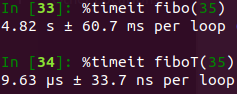
\includegraphics[width=0.4\linewidth]{screenshot001}
	\label{fig:screenshot001}
\end{figure}


\end{frame}

\begin{frame}{Összegzés}
	\begin{itemize}
		\item A bináris keresőfák műveletei $O(h)$ idejűek
		\item Legrosszabb esetben azonban $n$ is lehet a fák magassága ($\Theta(\log n)$ helyett)
		\item Kiegyensúlyozott keresőfák használatával garantálható, hogy a keresőfa kiegyensúlyozottsága sose romoljon el ''túlságosan''
	\end{itemize}
\end{frame}

\end{document}